%%%%
\newcommand{\elementText}[3]
{
  \begin{minipage}{2.2cm}
    \begin{center}
      \element{#1}{#2} % element symbol and atomic number
      \\[8 pt]
      \small{#3} % element name
    \end{center}
  \end{minipage}
}

%%%%
\newcommand{\tableauPeriodique}{
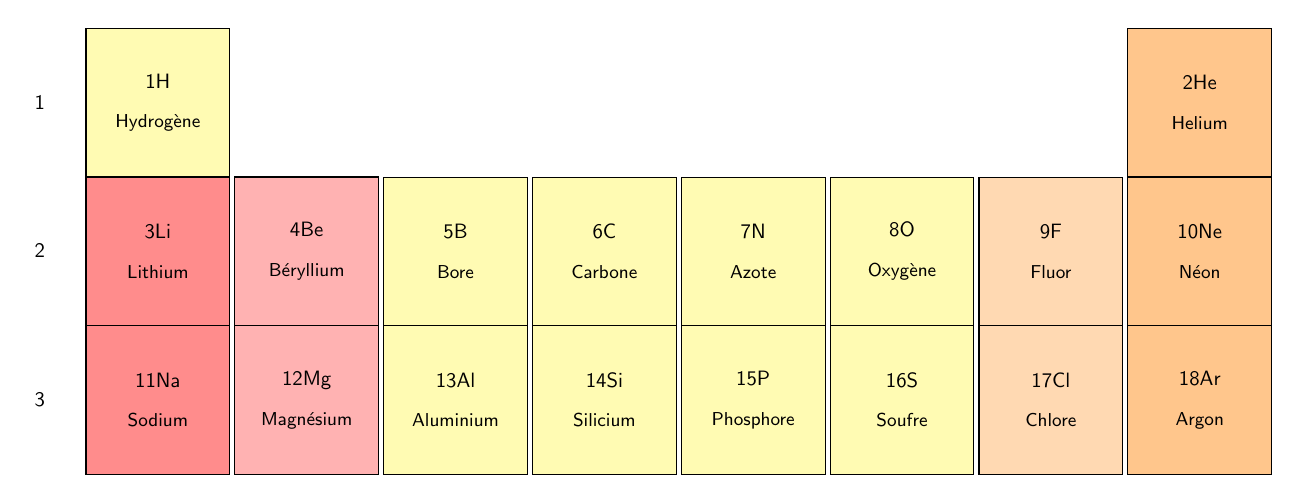
\begin{tikzpicture}[font=\sffamily, scale=0.75, transform shape]
%% Fill Color Styles
  \tikzstyle{elementFill}     = [fill=yellow!30]
  \tikzstyle{alkaliFill}      = [fill=red!45]
  \tikzstyle{alkaliEarthFill} = [fill=red!30]
  \tikzstyle{metalFill}       = [fill=red!15]
  \tikzstyle{metalloidFill}   = [fill=yellow!15]
  \tikzstyle{nonmetalFill}    = [fill=orange!15]
  \tikzstyle{halogenFill}     = [fill=orange!30]
  \tikzstyle{nobleGasFill}    = [fill=orange!45]

%% Element Styles
  \tikzstyle{Element} = [
    draw=black, elementFill,
    minimum width=2.25cm, minimum height=2.51cm,
    node distance=2.52cm
  ]
  \tikzstyle{Alkali}      = [Element, alkaliFill]
  \tikzstyle{AlkaliEarth} = [Element, alkaliEarthFill]
  \tikzstyle{Metal}       = [Element, elementFill]
  \tikzstyle{Metalloid}   = [Element, elementFill]
  \tikzstyle{Nonmetal}    = [Element, elementFill]
  \tikzstyle{Halogen}     = [Element, halogenFill]
  \tikzstyle{NobleGas}    = [Element, nobleGasFill]
  \tikzstyle{PeriodLabel} = [font={\sffamily\LARGE}, node distance=2cm]
  \tikzstyle{GroupLabel}  = [font={\sffamily\LARGE}, minimum width=2.5cm, node distance=2cm]
  \tikzstyle{TitleLabel}  = [font={\sffamily\Huge\bfseries}]

%% Group 1 - IA
  \node[name=H, Element]              {\elementText{1} {H} {Hydrogène}};
  \node[name=Li, below of=H, Alkali]  {\elementText{3} {Li}{Lithium}};
  \node[name=Na, below of=Li, Alkali] {\elementText{11}{Na}{Sodium}};
%% Group 2 - IIA
  \node[name=Be, right of=Li, AlkaliEarth] {\elementText{4} {Be}{Béryllium}};
  \node[name=Mg, below of=Be, AlkaliEarth] {\elementText{12}{Mg}{Magnésium}};
%% Group 13 - IIIA
  \node[name=B,  right of=Be, Metalloid] {\elementText{5} {B} {Bore}};
  \node[name=Al, below of=B,  Metal]     {\elementText{13}{Al}{Aluminium}};
%% Group 14 - IVA
  \node[name=C,  right of=B, Nonmetal]  {\elementText{6} {C} {Carbone}};
  \node[name=Si, below of=C, Metalloid] {\elementText{14}{Si}{Silicium}};
%% Group 15 - VA
  \node[name=N, right of=C, Nonmetal] {\elementText{7} {N}{Azote}};
  \node[name=P, below of=N, Nonmetal] {\elementText{15}{P}{Phosphore}};
%% Group 16 - VIA
  \node[name=O, right of=N, Nonmetal] {\elementText{8} {O}{Oxygène}};
  \node[name=S, below of=O, Nonmetal] {\elementText{16}{S}{Soufre}};
%% Group 17 - VIIA
  \node[name=F,  right of=O, Halogen] {\elementText{9} {F} {Fluor}};
  \node[name=Cl, below of=F, Halogen] {\elementText{17}{Cl}{Chlore}};
%% Group 18 - VIIIA
  \node[name=Ne, right of=F,  NobleGas] {\elementText{10}{Ne}{Néon}};
  \node[name=Ar, below of=Ne, NobleGas] {\elementText{18}{Ar}{Argon}};
  \node[name=He, above of=Ne, NobleGas] {\elementText{2} {He}{Helium}};

%% Period
  \node[name=Period1, left of=H,  PeriodLabel] {\normalsize{1}};
  \node[name=Period2, left of=Li, PeriodLabel] {\normalsize{2}};
  \node[name=Period3, left of=Na, PeriodLabel] {\normalsize{3}};
\end{tikzpicture}
}
